\documentclass[12pt]{article}

\usepackage[margin=1in]{geometry}
\usepackage{amsmath}
\usepackage{amssymb}
\usepackage{bbm}
\usepackage{setspace}
\usepackage{booktabs}
\usepackage{graphicx}
\usepackage{color}
\definecolor{oucrimson}{RGB}{132,22,23}
\usepackage[colorlinks=true,
            urlcolor=oucrimson,
            linkcolor=black,
            citecolor=black]{hyperref}
%\doublespacing



% --------------------------------------------------
\title{Problem Set 6}
\author{Tristan Winkle}
\date{}

% --------------------------------------------------
\begin{document}
\maketitle
% --------------------------------------------------

% --------------------------------------------------
\section{Questions and Responses}
% --------------------------------------------------

\subsection*{Data Cleaning}
The data used in this problem set come from the Armed Conflict Location \& Event Data Project (ACLED) for Africa. The raw data are event-level observations containing information on the date, country, event type, and geographic location of each recorded event. I intend to link this with nighttime lights data to estimate the causal impact of infrastructure failure on civil unrest. The nighttime lights data is only available for 2012-2025. I cleaned the ACLED data by limiting the sample period to these years and only for events classified as ``Protests" and ``Riots".

\pagebreak

\subsection*{Table}

\begin{table}[!htbp]
\centering
\caption{Top 15 African Countries by Protest and Riot Events}
\vspace{0.5em}
\begin{minipage}{0.68\textwidth}
\centering
\begin{tabular}{lrrr}
\toprule
Country         & Protests  & Riots     & Total \\
\midrule
South Africa    & 11,617    & 11,789    & 23,406 \\
Nigeria         & 8,239     & 5,514     & 13,753 \\
Morocco         & 12,352    & 678       & 13,030 \\
Kenya           & 5,351     & 7,119     & 12,470 \\
Tunisia         & 8,250     & 2,480     & 10,730 \\
Algeria         & 8,846     & 860       & 9,706 \\
DRC             & 4,013     & 4,364     & 8,377 \\
Sudan           & 7,149     & 965       & 8,114 \\
Egypt           & 3,657     & 2,647     & 6,304 \\
Uganda          & 1,946     & 3,282     & 5,228 \\
Ethiopia        & 3,173     & 851       & 4,024 \\
Guinea          & 1,223     & 1,916     & 3,139 \\
Somalia         & 1,865     & 844       & 2,709 \\
Ghana           & 915       & 1,665     & 2,580 \\
Zimbabwe        & 978       & 1,435     & 2,413 \\
\bottomrule
\end{tabular}

\vspace{0.5em}
\footnotesize
\textit{Notes:} Counts are based on ACLED protest and riot events from 2012--2025.
\end{minipage}
\end{table}

\noindent Table 1 reports the 15 African countries with the highest total number of protest and riot events in the ACLED sample from 2012–2025. South Africa records the largest total, followed by Nigeria, Morocco, and Kenya, indicating that unrest events are concentrated in a relatively small set of countries. The table is useful because it identifies which countries drive the broader continental patterns in the data.

\pagebreak

\subsection*{Figures}

\begin{figure}[!htbp]
\centering
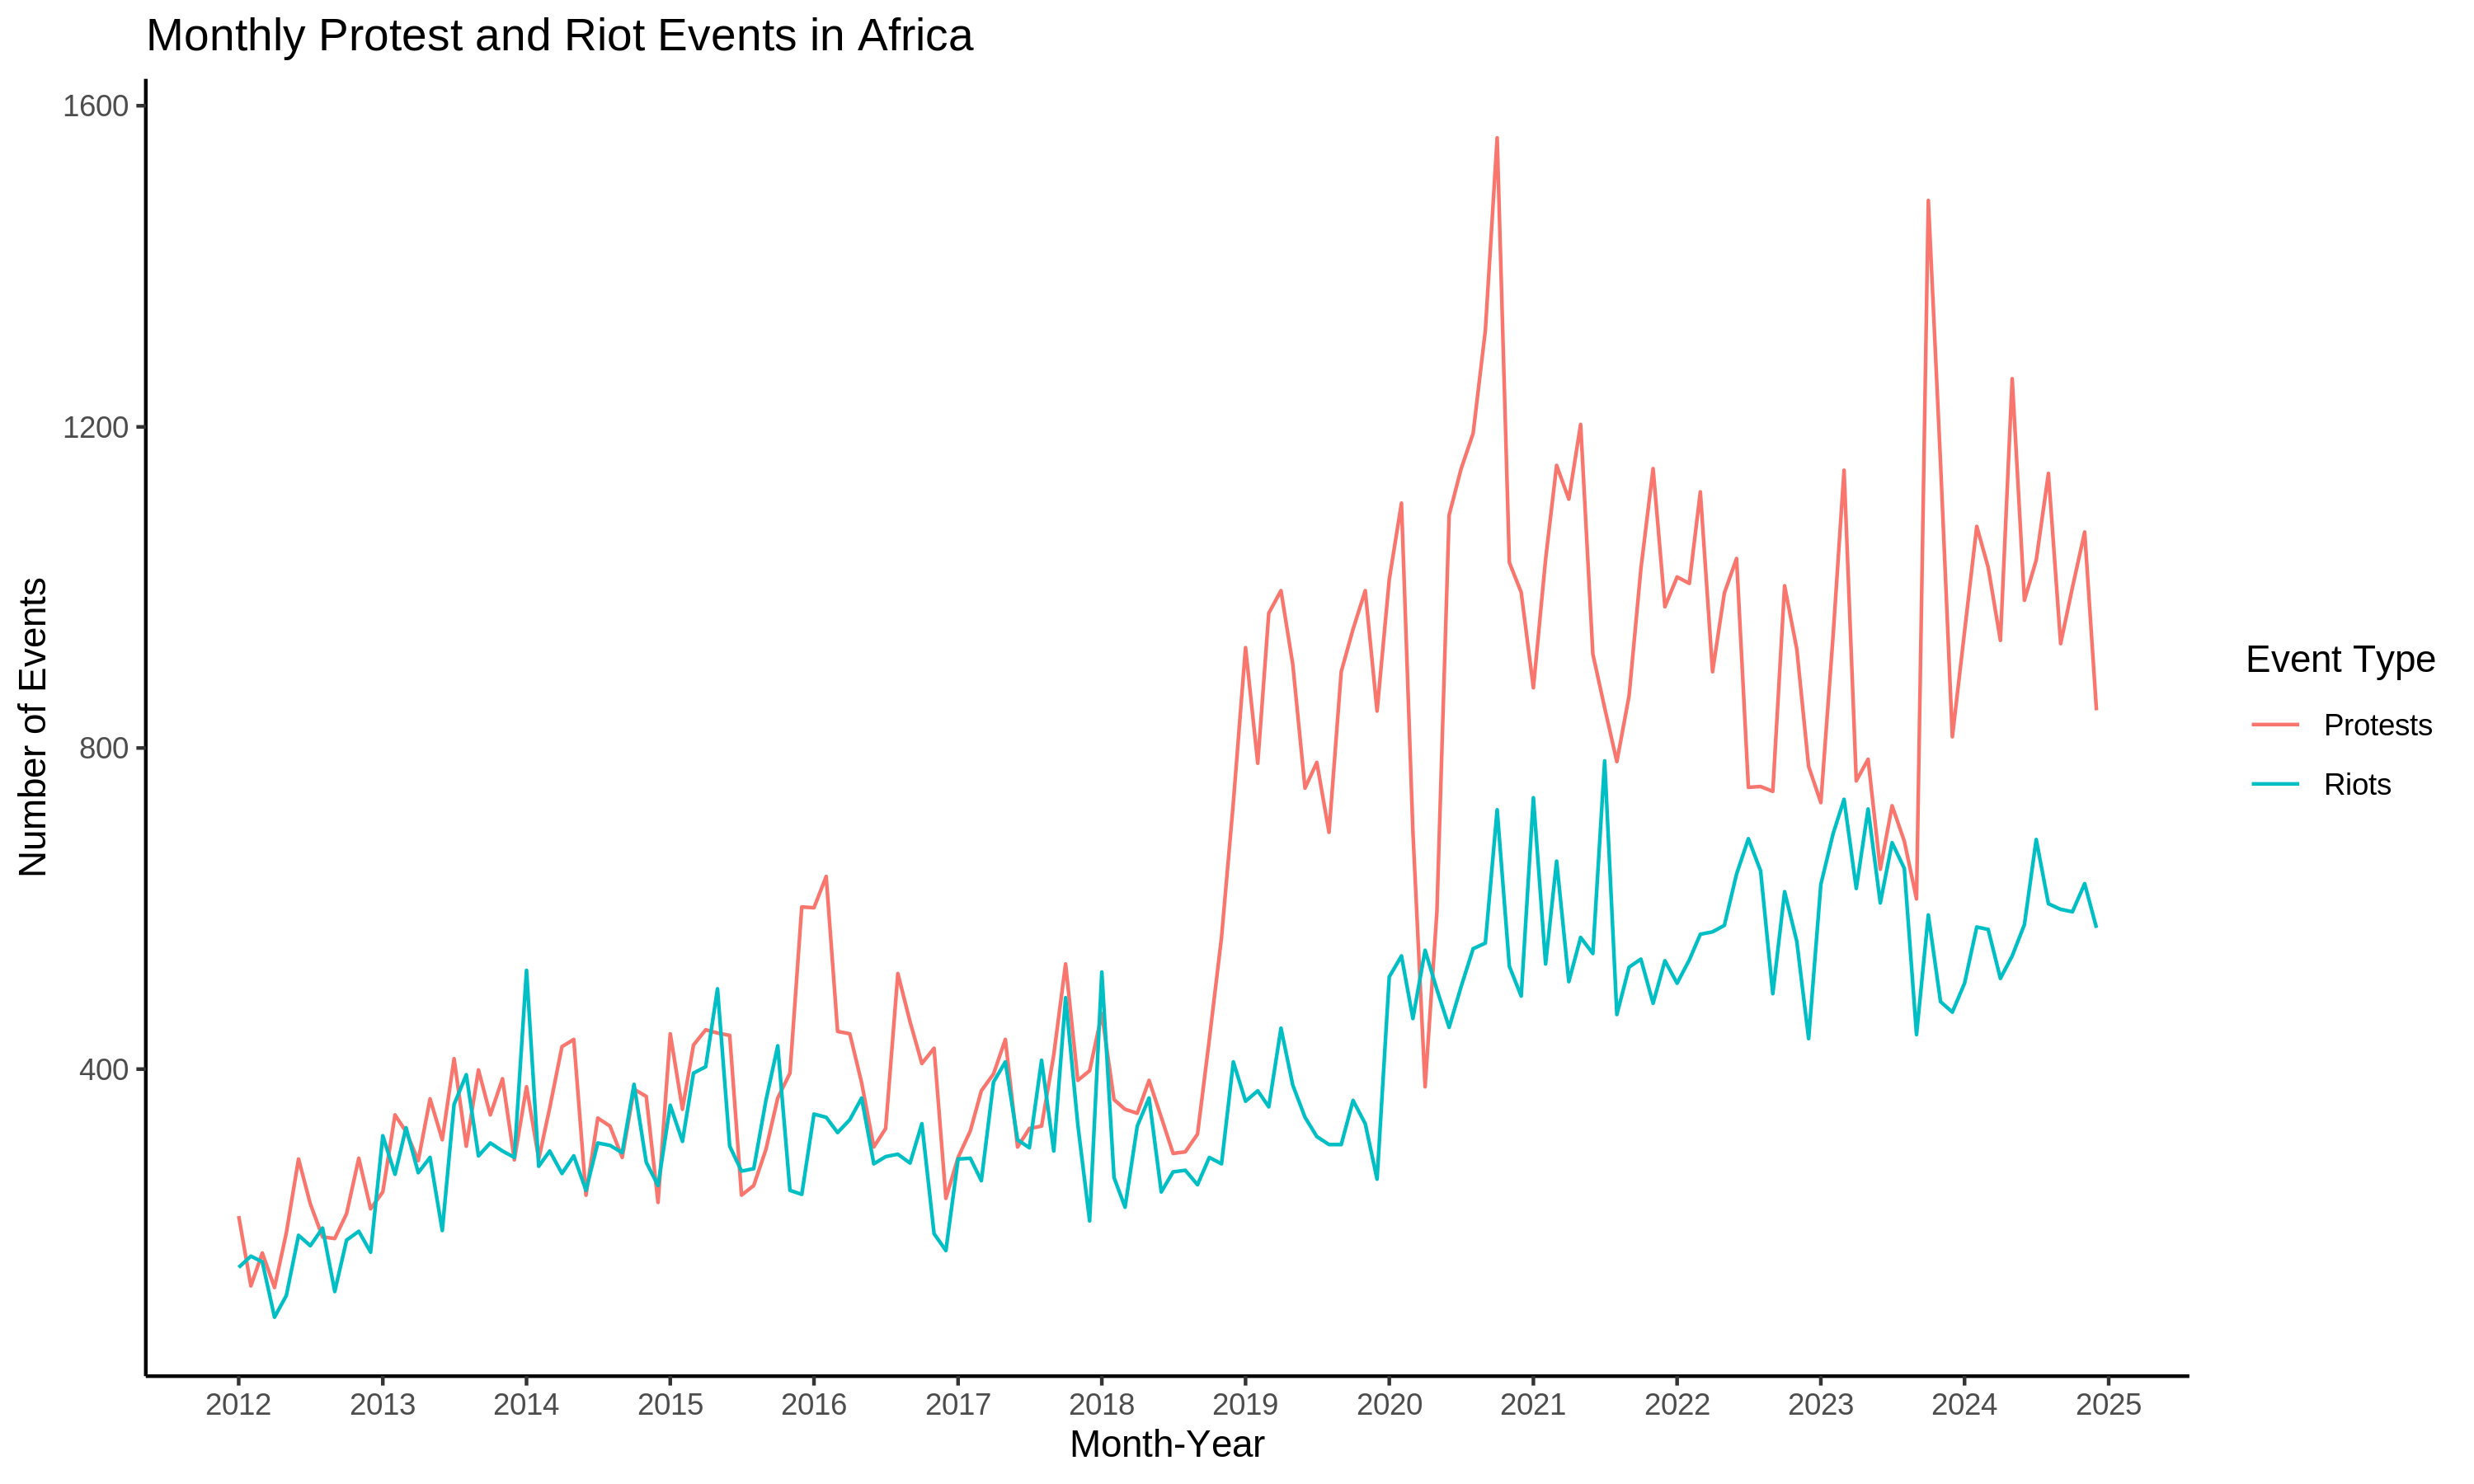
\includegraphics[width=0.9\textwidth]{PS6a_Winkle.png}
\caption{Monthly Protest and Riot Events in Africa}
\end{figure}

\noindent Figure 1 plots monthly protest and riot events in Africa from 2012–2025. Both series trend upward over time, but protests are consistently more frequent than riots, especially after 2019. The figure is useful because it provides a continent-level overview of unrest dynamics over the sample period.

\pagebreak

\begin{figure}[!htbp]
\centering
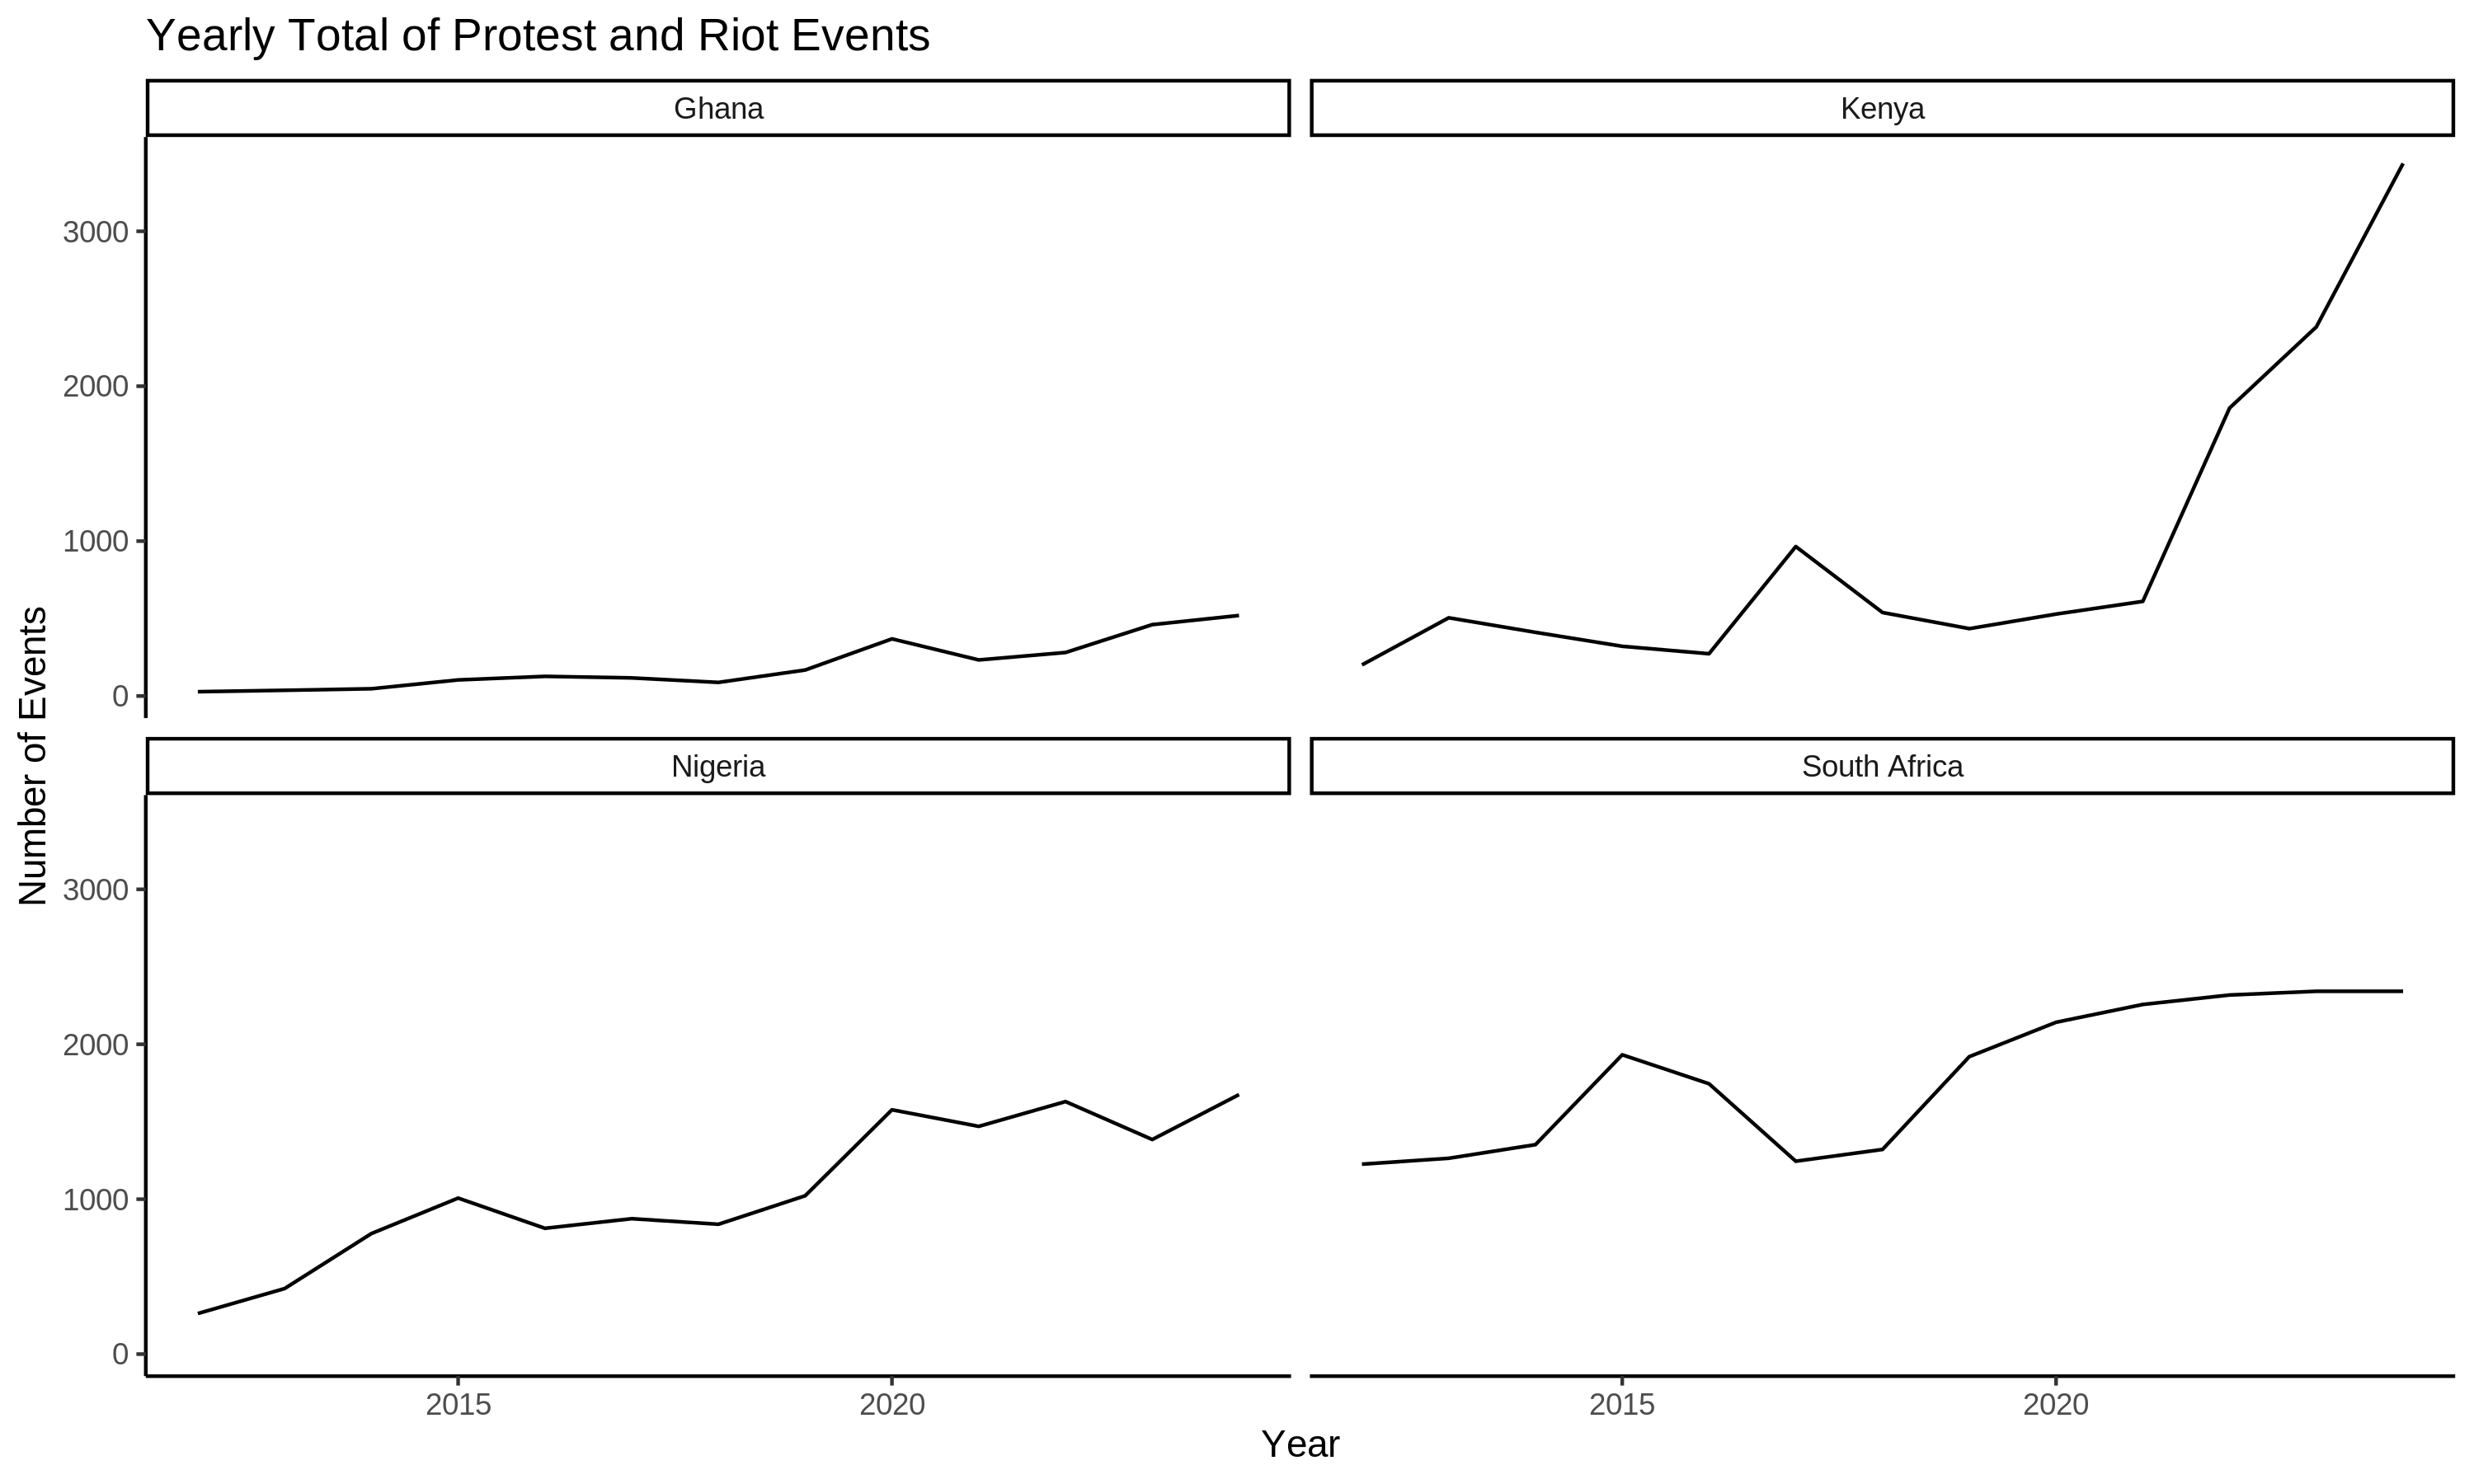
\includegraphics[width=0.95\textwidth]{PS6b_Winkle.png}
\caption{Yearly Protest and Riot Events in Countries with Frequent Infrastructure Failures}
\end{figure}

\noindent Figure 2 plots yearly total protest and riot events for Ghana, Kenya, Nigeria, and South Africa. The panels show clear cross-country heterogeneity: South Africa and Nigeria maintain high event counts throughout the sample, Kenya rises sharply in the most recent years, and Ghana remains lower overall. This comparison is useful because these countries also appear frequently in the development/energy economics literature on infrastructure failure and electricity reliability.



% --------------------------------------------------
\end{document}
% --------------------------------------------------
